%!TEX root=main.tex
\section{频偏估计}

\subsection{基本概念}
在时域接收到的信号为$y(t)=x(t) e^{j2 \pi \Delta f t}$,在频域为$Y = X(f - f')$。即时域旋转等价于频域移位。

粗频偏、细频偏应该是纠偏过程之中的概念,感觉两者没有什么实质差别,看的无非是一个纠偏精确度的问题;其实可以把粗频偏和细频偏合到一起做也可以的。当然纠偏也可以采用第一次纠偏之后再跟踪残余频偏的方式进行。
\begin{itemize}
\item 整数倍频偏和小数倍频偏是频偏大小的概念。一般用好的天线是不存在整数倍频偏的。整数倍频偏导致的是子载波数据的偏移,而小数倍频偏导致的是ICI。
\item 不能先进行整数倍频偏估计再进行小数倍频偏估计。因为一般整数倍频偏导致的是子载波数据的偏移,其估计方式是在频域估计;而小数倍频偏会导致ICI,使得频域数据无法提取。所以必须要先估计出小数倍频偏,消除了ICI,提取出频域子载波数据,然后再做整数倍频偏估计。
\end{itemize}


\subsection{802.11中频偏估计}
在802.11a/g/n中,使用legacy long training field(L-LTF)来估计$\Delta f_{ij}$。
$\Delta f_{ij} = -\frac{arg[ y(t - \delta t)y^{*}(t)  ]}{2 \pi \delta t}$, $\delta t = 3.2 \mu s$。$arg$被定义为$arctan$,其取值范围为$(-\frac{\pi}{2}, +\frac{\pi}{2})$。所以利用L-LTF估计的频偏范围为$(-78.125KHz, +78.125KHz)$。
子载波间隔为$\Delta f = \frac{20MHz}{64} = 312.5KHz$。

\subsection{频偏带来ICI}
发送的时域信号为$x=[x_{0}, x_{1}, \cdots, x_{63}]$,设频偏为$\Delta f$,则接收到的时域信号为
\begin{eqnarray}
r&=&[x_{0}e^{j\frac{2\pi*0\Delta f}{f_{s}}}, x_{1}e^{j\frac{2\pi*1\Delta f}{f_{s}}}, \cdots, x_{63}e^{j\frac{2\pi*63\Delta f}{f_{s}}}]
\end{eqnarray}
接收到的频域信号为$R=FFT(r)$。由于频偏的存在,FFT之后的结果中存在ICI。

As noted in (http://www.stanford.edu/$\sim$hsiying/pubs/globecom10-cdma\_ici.pdf), 
received signal on subcarrier $i$ in AWGN channel with ICI is
\begin{eqnarray}
R(i) & = & X(i)S(0) \\
      & + & \Sigma_{l=0, l \neq i}^{N-1} X(l)S(l-i) + n_{i} \\
      &     & i = 0, 1, \cdots, N-1 \nonumber
\end{eqnarray}
where N is the total number of subcarriers, $X(i)$ denotes the transmitted symbol, $n_{i}$ is the additive Gaussian noise on $i^{th}$ subcarrier. The sequence $S(l-i)$ is the ICI coefficient from $l^{th}$ subcarrier to $i^{th}$ subcarrier:
\begin{eqnarray}
S(l-i) & = & \frac{sin(\pi (\epsilon + l - i))}{N sin(\frac{\pi}{N}(\epsilon + l - i))} \\
         & \cdot  & exp( j\pi (1 - \frac{1}{N})(\epsilon + l - i))
\end{eqnarray}
where $\epsilon$ is the normalized frequency offset given by $\epsilon = \frac{\Delta f}{\Delta F}$, $\Delta F$ is the subcarrier bandwidth, $\Delta f$ is the carrier frequency offset.
$S(0)$对于$X(i)$的影响在于幅度的减小和相位的旋转。当$\epsilon$很小是可以忽略ICI,认为ICI为噪声。

\subsection{频偏造成旋转}
设$\Delta f$是频偏,估计在$t$时间后旋转多少度
\begin{eqnarray}
\theta & = & \frac{2 \pi \Delta f t}{\pi} \cdot 180 \\
           & = & 360 \cdot \Delta f \cdot t
\end{eqnarray}
假设$\Delta f =  10 KHz$, $t=4 * 10^{-9}s$,那么旋转过的角度为$0.0144$度,即在一个OFDM Symbol内,可以认为不旋转,相邻两个OFDM Symbol之间的相位差可以忽略,这样在估计信道的时候,相位带来的影响就很小了。


在802.11中,使用L-LTF来估计$\Delta f$,估计出来的值会不准确,有一定的方差。
比如已知$\Delta f = 80 KHz$,在固定噪声的情况下进行多次估计,得到的估计值$\Delta \hat{f}$符合均值为80KHz,方差为$\sigma$($\sigma$取决于SNR)的均匀分布(Figure \ref{fig:cfovar})。
\begin{figure}
	\centering
	\begin{tabular}{ccc}
		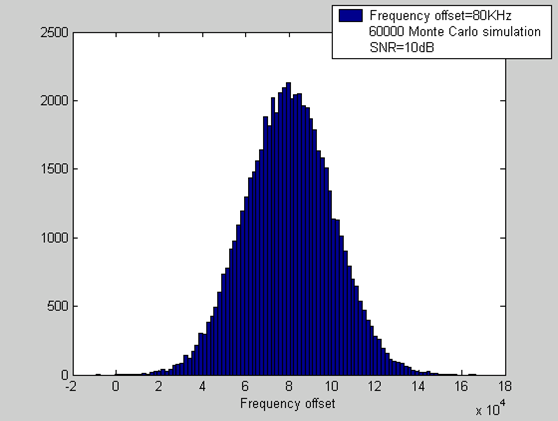
\includegraphics[width=0.3\textwidth]{SimCFO1.png} &
		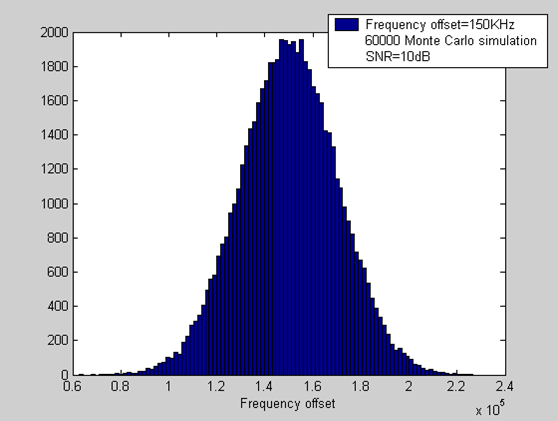
\includegraphics[width=0.3\textwidth]{SimCFO2.png} &
		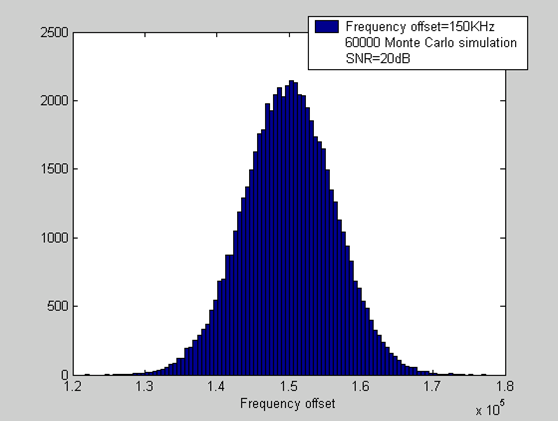
\includegraphics[width=0.3\textwidth]{SimCFO3.png}
	\end{tabular}
	\caption{频偏估计误差}\label{fig:cfovar}
\end{figure}


%
\subsection{多用户频偏估计}
假设有M个发送端(STA),N个接收端(AP),各自的中心频率不相同。
设$\Delta f_{ij}$为$STA_{j}$与$AP_{i}$之间的频偏。

以2x2为例,每个用户频域上有4个pilot,用户$i$的pilot分别为$p_{i,-21}$,$p_{i,-7}$,$p_{i,7}$,$p_{i,21}$,在$t$时刻接收端$i$在第$k$个pilot上收到到的信号为$y_{i, k}^{t}$
\begin{eqnarray}
y_{1, -21}^{t} & = & h_{11,-21}^{t}f_{11}p_{1,-21} + h_{12,-21}^{t}f_{12}p_{2,-21} \\
y_{2, -21}^{t} & = & h_{21,-21}^{t}f_{21}p_{1,-21} + h_{22,-21}^{t}f_{22}p_{2,-21} \\
y_{1, -7}^{t}   & = & h_{11,-7}^{t}f_{11}p_{1,-7} + h_{12,-7}^{t}f_{12}p_{2,-7} \\
y_{2, -7}^{t}   & = & h_{21,-7}^{t}f_{21}p_{1,-7} + h_{22,-7}^{t}f_{22}p_{2,-7} \\
y_{1, 7}^{t}   & = & h_{11,7}^{t}f_{11}p_{1,7} + h_{12,7}^{t}f_{12}p_{2,7} \\
y_{2, 7}^{t}   & = & h_{21,7}^{t}f_{21}p_{1,7} + h_{22,7}^{t}f_{22}p_{2,7} \\
y_{1, 21}^{t} & = & h_{11,21}^{t}f_{11}p_{1,21} + h_{12,21}^{t}f_{12}p_{2,21} \\
y_{2, 21}^{t} & = & h_{21,21}^{t}f_{21}p_{1,21} + h_{22,21}^{t}f_{22}p_{2,21}
\end{eqnarray}
解上述方程可得$f_{11}$,$f_{12}$,$f_{21}$,$f_{22}$。

更新$t+1$时刻第$k$个子载波的信道$h_{ij, k}^{t+1}$:
\begin{eqnarray}
h_{11, k}^{t+1} & = & h_{11,k}^{t}f_{11} \\
h_{12, k}^{t+1} & = & h_{12,k}^{t}f_{21}\\
h_{21, k}^{t+1} & = & h_{11,k}^{t}f_{11} \\
h_{22, k}^{t+1} & = & h_{12,k}^{t}f_{21}
\end{eqnarray}










